\section{热机和环境保护}\label{sec:6-4}

热机的广泛应用,促进了社会生产的发展和人们生活水平的提高。
但是,任何事物都有两面性,热机的大量应用,也会污染环境,给人们带来危害。

热机工作时往往产生很大的噪声。
火车的轰隆声,城市中大量汽车产生的噪声,干扰了人们的正常工作和生活。
热机工作都要消耗燃料,燃料燃烧过程中,会排出二氧化硫、氮氧化合物、一氧化碳、
二氧化碳以及飞灰等物质。这些物质对人体的健康有害。

环境污染问题,在一些工业发达的国家里,在五十年代就成了社会公害。
目前,世界各国对控制污染、保护环境都十分重视,在这方面进行了大量的研究工作,
并采取了许多保护环境的措施。

随着工业建设的发展,我国也出现了环境污染问题。
党和政府对保护环境和人民健康十分关心,已经建立了专门机构,研究解决这些问题。
我们要做到:既要发展生产,又要保护好祖国的壮丽河山,使人民有一个清洁美好的生活环境。




\section*{阅读材料:热机的发展}

\begin{wrapfigure}{r}{7cm}
    \centering
    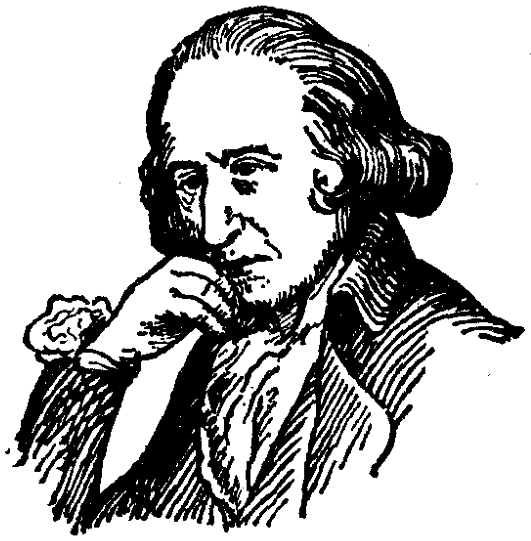
\includegraphics[width=6cm]{../pic/czwl2-ch6-watt}
    \caption*{瓦特(1736 ~ 1819)}\label{fig:6-watt}
\end{wrapfigure}

十七世纪以前,人们的生产活动除了用人力、畜力外,只能利用风力、水力来带动一些简单机械。
从十七世纪起,随着生产的发展,特别是纺织机等的陆续出现,人力、畜力、风力、水力不能满足需要了。
同时,机器制造业已经产生,使发明、制造新的动力机成为可能。

世界上最早的热机——蒸汽机就是在这种情况下发明的。
蒸汽机先后经过许多人的研究、试制和改进,其中贡献最大的是英国的工人出身的技师瓦特。
1782 年,他发明了往复式蒸汽机,使蒸汽机逐步成为一种广泛应用的动力机。

% \begin{figure}[htbp]
%     \centering
%     \begin{minipage}{4cm}
%     \centering
%     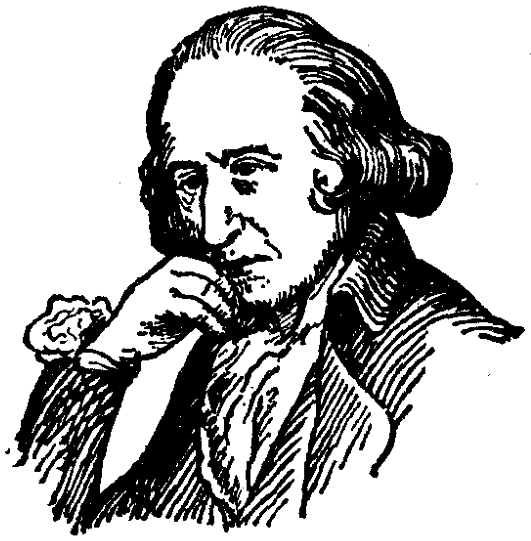
\includegraphics[width=4cm]{../pic/czwl2-ch6-watt}
%     \caption*{瓦特(1736 ~ 1819)}\label{fig:6-watt}
%     \end{minipage}
%     \qquad
%     \begin{minipage}{10cm}
%     \centering
%     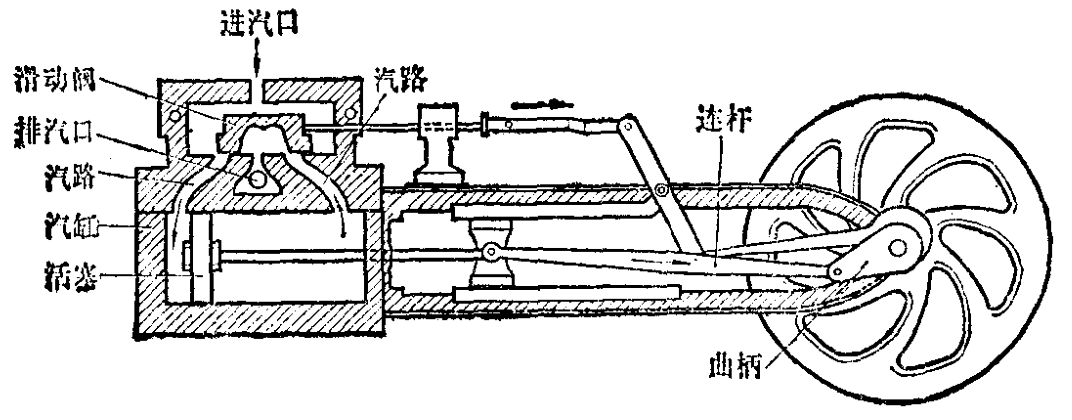
\includegraphics[width=10cm]{../pic/czwl2-ch6-3}
%     \caption{往复式蒸汽机示意图}\label{fig:6-3}
%     \end{minipage}
% \end{figure}

图 \ref{fig:6-3} 是往复式蒸汽机的示意图。
由锅炉来的
高温高压蒸汽进入汽缸  左侧,推动活塞向右运动。活塞右侧的废汽经右侧的汽路从排汽口排出。
当活塞运动到右端时,滑动阀遮住左侧的汽路,
高温高压蒸汽进入汽缸的右侧,推动活塞向左运动,活塞左侧的废汽经左侧的汽路从排汽口排出。
这样,蒸汽使活塞不停地做往复运动。活塞的往复运动,通过连杆、曲柄,使机轴和飞轮转动。

\begin{figure}[htbp]
    \centering
    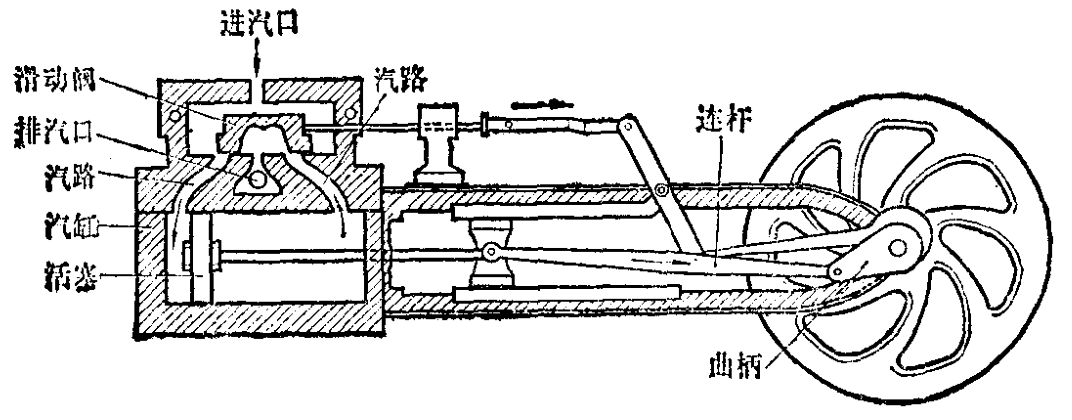
\includegraphics[width=0.8\textwidth]{../pic/czwl2-ch6-3}
    \caption{往复式蒸汽机示意图}\label{fig:6-3}
\end{figure}

蒸汽机的发明对当时工业发展起了巨大的作用。
但是,蒸汽机需要庞大的锅炉生产水蒸气,还需要曲柄连杆机构把往复运动变为转动,
这就使蒸汽机十分笨重,而且效率很低,只有 6 ~ 15 \% 。
为了克服这些缺点,人们发明了不要锅炉设备的内燃机和不要曲柄连杆机构的蒸汽轮机。

属于内燃机的汽油机是在 1876 年发明的,柴油机是在 1892 年发明的。
内燃机体积小,使用起来比蒸汽机方便多了。
内燃机发明后,汽车、飞机出现了,用在农业上的拖拉机也出现了。
内燃机的广泛应用,对生产技术的发展起了很大的促进作用。

蒸汽轮机是 1884 年出现的,它的基本特点是让锅炉里来的高温高压蒸汽从喷嘴高速喷出,
冲击叶轮的叶片,直接使机轴转动(图 \ref{fig:6-4})。
蒸汽轮机的效率比蒸汽机高得多,一般是 25 ~ 30 \%。
目前大型火力发电站大多采用蒸汽轮机。现代的蒸汽轮机的功率达到几十万千瓦。

\begin{wrapfigure}{r}{7cm}
    \centering
    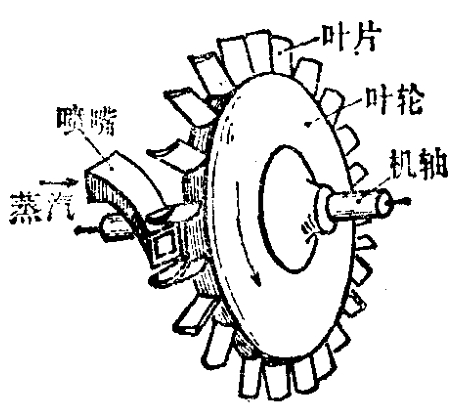
\includegraphics[width=6cm]{../pic/czwl2-ch6-4}
    \caption{}\label{fig:6-4}
\end{wrapfigure}

最近几十年来,人们吸取内燃机和蒸汽轮机的特点,研制成了燃气轮机。
它是让高温高压的燃气直接冲击叶轮的叶片而做功的,它没有笨重的锅炉设备,也不用曲柄连杆机构。
因此,燃气轮机的体积小、重量轻、效率高(可以达到 50 ~ 60 \% )。
但是,燃气轮机让高温高压的燃气直接冲击叶片,这就要求使用性能优良的耐热材料来制造叶片,
而且要有很好的冷却设备,以保证机器在工作中不致过热。
燃气轮机首先应用在飞机上,目前在火车和火力发电站上也已开始试用。

现代喷气式飞机上应用的发动机是一种新型的热机——空气喷气发动机。
喷气发动机是让高温高压的燃气高速地向后喷出,而使发动机获得向前的动力。
空气喷气发动机需要利用空气中的氧气来帮助燃料燃烧,因此,
使用这种热机的飞行器不能飞到大气层以外的空间里去。
另外还有一种喷气发动机,它既带燃料,又带氧化剂,不需要空气中的氧气助燃。
这种发动机就是火箭喷气发动机,常简称火箭。
火箭是人类征服宇宙空间的工具,人造地球卫星就是用火箭发射的。

从蒸汽机出现以来,热机已经发展到了很高的水平。
但是事物总是不断发展的,随着科学技术水平的提高,必定会有更好、更新的热机出现,为人们的生产和生活带来更多的方便。

